\scanpage{62}
\mspage{30}
la courbe modulaire $\unsure{\widehat{\mathcal X}^!_{0,4}|\widehat{\mathfrak X}^!_{0,4}}$ sur $\widehat M^!_{0,4}$, avec ses quatre sections $s_0,s_1,s_\infty,s_\lambda$ (ou $t_1,t_2,t_3,t_4$), et avec l'opération de $\mathfrak S_4$ \deleted{dessus} sur $\unsure{\widehat{\mathcal X}^!_{0,4}|\widehat{\mathfrak X}^!_{0,4}}\longrightarrow\widehat M^!_{0,4}$, échangeant ces quatre sections entre elles. Je vais pas le faire ici --- cela donnera du $=$ coup les \deleted{\unsure{schémas}}\inserted{multiplicités} modulaires $\widehat M_{0,4}$ et $\unsure{\widehat{\mathcal X}_{0,4}|\widehat{\mathfrak X}_{0,4}}$. Pour $\widehat M_{0,4}$, il y a lieu de remplacer le diagramme (76) par un diagramme purement numérique
\figure{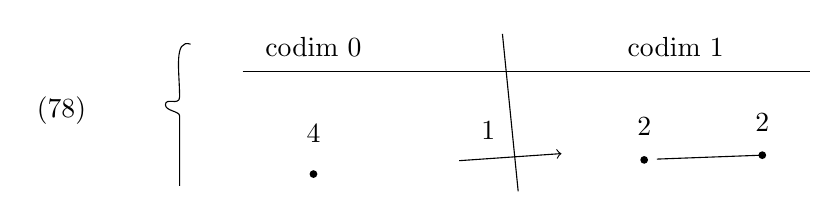
\begin{tikzpicture}[x=1cm,y=1cm]
\node at (-3.2,.8) {$(78)$};
\draw (-1.56,1.65) .. controls (-1.78,1.72) and (-1.70,1.30) .. (-1.70,.98) .. controls (-1.70,.86) and (-1.88,.98) .. (-1.88,.88) .. controls (-1.88,.80) and (-1.70,.80) .. (-1.70,.74) -- (-1.70,-.15);
\draw (-.9,1.30)--(6.3,1.30);
\draw (2.4,1.78)--(2.6,-.22);
\node at (0,1.62) {codim $0$};
\node at (4.6,1.62) {codim $1$};
\fill (0,0) circle (1.4pt);
\node[above] at (0,.28) {$4$};
\draw[->] (1.85,.17)--(3.15,.26);
\node[above] at (2.22,.31) {$1$};
\fill (4.2,.18) circle (1.4pt);
\fill (5.7,.24) circle (1.4pt);
\draw (4.36,.19)--(5.7,.24);
\node[above] at (4.2,.36) {$2$};
\node[above] at (5.7,.42) {$2$};
\end{tikzpicture}}
il n'y a plus qu'un seul pt à l'infini, correspondant aux trois pts à l'infini de $\widehat M^!_{0,4}$, permutés transitivement entre eux par $\mathfrak S_4$.

Caractéristiques d'EP fractionnaires. On trouve
\[
\begin{aligned}
\chi_!(M^{!\,\mathrm{an}}_{0,4})&=\chi_!(U^{\mathrm{an}}_{0,3})=2-2\underset{\substack{\Vert\\0}}{g}-\underset{\substack{\Vert\\3}}{\nu}=-1\\
\chi_!(\widehat M^{!\,\mathrm{an}}_{0,4})&=\chi_!(\mathbb P^{1\,\mathrm{an}})=2\\
\chi_!(\overset{\deleted{\unsure{\widehat{\phantom M}\,!}}}{M}{}^{\mathrm{an}}_{0,4})&=\chi_!(\unsure{U|\mathbb P}^{\mathrm{an}}_{0,3},\mathfrak S_4)\\
&=\chi_!\bigl(U^{\mathrm{an}}_{0,3}\smallsetminus\{-\bar j,-j\}\smallsetminus\{\tfrac12,2,-1\},\mathfrak S_4\bigr)\\
&\qquad+\chi_!(\{-\bar j,-j\},\mathfrak S_4)+\chi_!(\{\tfrac12,2,-1)\mathfrak S_4)\\
&=-1+\frac13+\frac12=-\frac1{\unsure{24|6}}
\end{aligned}
\]
\margin{\uline{NB} On peut écrire directement $\chi_!(U^{\mathrm{an}}_{0,3}):[\mathfrak S_4]=-\frac1{24}$}
\margin{61}
